
\section{Чудеса теории вероятностей}
Чудо 1. <<Гороскоп>>\\
У тёти Глаши двое детей.
\begin{enumerate}
\item  Оценить вероятность того, что у нее два сына, при условии, что у хотя бы один из ее детей --- мальчик.
Находим просто по формуле (M --- мальчик, D --- девочка):
$p(MM|\bar{DD})=\frac{p(MM,\bar{DD}}{p(\bar{DD})}=\frac{1/4}{3/4}=\frac{1}{3}$
\item Оценить вероятность того, что у нее два сына, при условии, что у хотя бы один мальчик --- стрелец.
Построим дерево судьбы тети Глаши(MC --- мальчик-стрелец, МНС --- мальчик-не стрелец):
\end{enumerate}

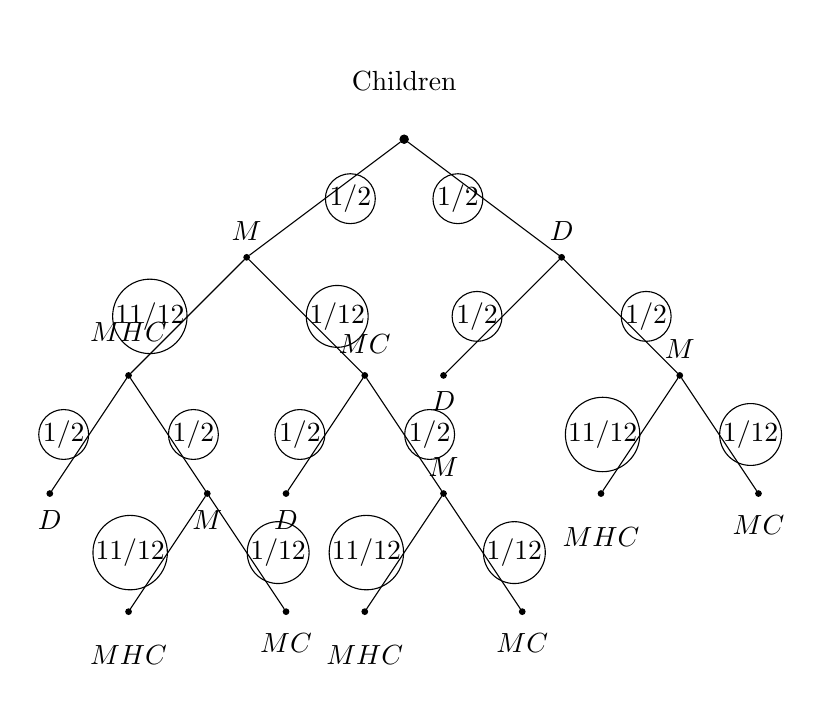
\begin{tikzpicture}[grow=down]
 \tikzset{edge from parent/.style=
     {draw, edge from parent path={(\tikzparentnode) -- (\tikzchildnode)}}}
\tikzstyle{mystart} = [circle, minimum width=3pt,fill, inner sep=0pt]
\tikzstyle{mydot} = [circle, minimum width=2pt,fill, inner sep=0pt]
\tikzstyle{level 1}=[sibling distance=4cm]
\tikzstyle{level 2}=[sibling distance=3cm]
\tikzstyle{level 3}=[sibling distance=2cm]

\node[mystart, label=above: {Children}] {} 
	child { node[mydot, label=above: $M$] {}
		child { node[mydot, label=above: $MHC$] {}
			child { node[mydot, label=below: $D$] {}
			edge from parent node[left] {$1/2$} }
			child { node[mydot, label=below: $M$] {}
				child { node[mydot, label=below: $MHC$] {}
				edge from parent node [left] {$11/12$} }
				child { node[mydot, label=below: $MC$] {}
				edge from parent node [right] {$1/12$} }
			edge from parent node[right] {$1/2$} }
		edge from parent node[left] {$11/12$} }
		child { node[mydot, label=above: $MC$] {}
			child { node[mydot, label=below: $D$] {}
			edge from parent node[left] {$1/2$} }
			child { node[mydot, label=above: $M$] {}
				child { node[mydot, label=below: $MHC$] {}
				edge from parent node [left] {$11/12$} }
				child { node[mydot, label=below: $MC$] {}
				edge from parent node [right] {$1/12$} }
			edge from parent node[right] {$1/2$} }
		edge from parent node[right] {$1/12$} }
	edge from parent node[right] {$1/2$} }
	child { node[mydot, label=above: $D$] {}
		child { node[mydot, label=below: $D$] {}
		edge from parent node[left] {$1/2$} }
		child { node[mydot, label=above: $M$] {}
			child { node[mydot, label=below: $MHC$] {}
			edge from parent node [left] {$11/12$} }
			child { node[mydot, label=below: $MC$] {}
			edge from parent node [right] {$1/12$} }
		edge from parent node[right] {$1/2$} }
	edge from parent node[left] {$1/2$} };
\end{tikzpicture}

Теперь вспомним, что вероятность исхода на дереве равна произведению вероятностей на веточках, ведущих к этому исходу. Найдем нужные ветви судьбы, где у тети Глаши рождается два сына и где один мальчик --- стрелец, и посчитаем:
$p(MM|\exists {MC})=\frac{p(MM,\exists{MC})}{p(\exists {MC})}=\frac{1/12*1/12*1/2+1/2*11/12*1/2*1/12}{1/12*1/12*1/2+1/2*11/12*1/2*1/12+1/2*1/12*1/2+1/2*1/2*1/12}=\frac{23}{47}$
Чудо! Вероятность двух сыновей при условии, что один сын --- стрелец, почти $1/2$!
Почему так происходит? Потому что рождение стрельца --- куда более редкое событие, чем рождение просто мальчика.
end{enumerate}

Чудо 2. <<Два конверта>>\\
Вам предлагают два конверта. Известно, что суммы денег в них относятся как 1:2. Вы открыли один конверт, и увидели в нём 100 рублей. Вопрос: стоит ли поменять выбор конверта?
А непонятно: мы не знаем закон распределения. 
Допустим, у нас такое распределение:
$\begin{array}{c|ccc}
\hline
(X;Y) & {25;50} & {12,5;25} & {50;100} \\
\P() & 1/3 & p {1/3} & {1/3} \\
\end{array}$ \\
Тогда $\E(Y|X=100)=50$, и мы не будем менять конверт. Но в другом распределении, где, к примеру, вместо исхода $(25;50)$ был бы исход $(100;300)$, наш ожидаемый выигрыш от смены конверта был бы 175, и мы бы поменяли. 

Чудо 3.  <<Спящая Красавица>>\\
Спящая Красавица согласилась на участие в научном эксперименте. 
Протокол научного эксперимента:
\begin{enumerate}
\item Ее колют веретеном в воскресенье.
\item После укола веретеном подкидывают монетку.
\item В понедельник ее будят и задают вопрос. Если монетка в воскресенье выпала орлом, ее отпускают, если решка --- снова колют веретеном.
\item Во вторник ее снова будят и задают тот же вопрос, но из-за психотропного вещества на конце веретена она не помнит, сколько раз она просыпалась. 
\end{enumerate}
Спросить ее могут:
\begin{itemize}
\item Какова вероятность того, что сегодня понедельник?
\item Как выпала монетка?
\item Какой сегодня день недели?
\end{itemize}
 Как Спящей красавице нужно отвечать на вопросы?

Неясно. Первый вопрос вообще сформулирован некорректно: <<сегодня понедельник>> --- это не событие, а функция от времени: $f(t=$пн$)=TRUE$ или $f(t=$пн$)=FALSE$.
А на другие вопросы она отвечать каким-либо определенным образом не заинтересована. \\

Пусть теперь в эксперименте предусмотрена система поощрений: за каждый правильный ответ Спящей Красавице будут дарить молодильное яблоко. 
Условимся для краткости называть случай с выпадением орла первым сценарием, решки --- вторым.
Тогда если она ответит <<орел>>, то в первом сценарии она получит 1 яблоко, во втором --- 0.
Если же она ответит <<решка>>, то в первом сценарии она ничего не получит, а во втором получит 2 яблока.
Понятно, что выгоднее ей будет ответить <<решка>>.

Система поощрений поменялась, и теперь за каждый неправильный ответ Спящую Красавицу превращают в тыкву.
Если она в таком случае ответит <<орел>>, то в первом сценарии она выживет, во втором --- погибнет, с равными вероятностями. Если Красавица выберет <<решку>>, то в первом сценарии она  погибнет, а во втором --- выживет, опять с равными вероятностями. Так что при такой системе ей все равно, что отвечать.
Вот и чудо: ответ на один и тот же вопрос меняется в зависимости от системы поощрений.

На вопрос, какой сегодня день недели, ответ нужно тоже смотреть в зависимости от системы поощрений. Если за каждый правильный ответ дарят молодильное яблоко, то выгоднее отвечать понедельник (и в первом, и втором сценарии она получит по одному яблоку). Правда, если за каждый неправильный ответ превращают в тыкву, то все равно выгоднее отвечать понедельник (в таком случае ее хотя бы отпустят в первом сценарии, а во втором --- превратят в тыкву, а если она будет отвечать <<вторник>>, то превратится в тыкву в любом случае).

Чудо 4. Игра Паррондо(Parrondo'sgame, 1996)\\
Есть две игры:
Игра А: выиграть 1 рубль с вероятностью 0.45 или проиграть 1 рубль с вероятностью 0.55. Видно, что игра А --- проигрышная.\\
Игра В: Вы показываете содержимое вашего кошелька. Если сумма в Вашем кошельке делится на три, то вы получаете 1 рубль с вероятностью 0.05 и теряете рубль с вероятностью 0.95; если не делится --- получаете рубль с вероятностью 0.7; проигрываете рубль --- с вероятностью 0.3.

Задание:
\begin{enumerate}
\item Игра В --- проигрышная, надо это доказать.
\item Ответить, что происходит с благосостоянием, если долго играть в игру В.
\item С вероятностями 1/2 и 1/2 играем в игры А и В: каждый раз подкидываем монетку и решаем, во что будем играть. Такая игра окажется выигрышной.
\end{enumerate}

Задача --- на дом. Здесь наметки:
Поделим возможные суммы в кошельке на тройки (для упрощения предположим еще, что мы можем уходить в минус --- брать кредит). Вертеться в стартовой тройке бесконечно нельзя: рано или поздно с вероятностью 1 вылетим из нее. Строим сетку, как мы можем ходить по тройкам с разных стартовых элементов. 

\section{Условная независимость}

<<Классическая>> независимость событий $A$ и $B$: $\P(AB)=\P(A)*\P(C)$
Условная независимость. События $A$ и $B$ называются условно независимыми при условии, что событие $C$ произошло, если $\P(AB \mid C)=\P(A \mid C)\P(B \mid C)$ или, что эквивалентно, $\P(A\mid BC)=\P(A\mid C)$. 

Примеры.
\begin{enumerate}
\item Независимые, но условно зависимые события.
Монетку подбросили два раза. $A$ --- выпал орел в первый раз, $B$ --- выпал орел во второй раз, $C$ --- выпал всего один орел. $A$ и $B$ независимы, но $\P(A\mid B\cap C)=0$, а $\P(A\mid C)=1/2$: нет условной независимости.
\item Зависимые, но условно независимые события.
$A$ --- Маша идет в кино, $B$ --- Саша идет в кино, $C$ --- они не знакомы.\\

Есть правильная монетка (1/2 --- орел) и неправильная монетка (2/3 --- орел). Мы выбираем монетку с вероятностью 1/2 и подбрасываем 2 раза (одну и ту же). $A$ --- в первый раз орел, $B$ --- орел во второй раз, $C$ --- была выбрана неправильная монетка.\\
$\P(A)=1/2*1/2+1/2*2/3=7/12$\\
$\P(A\mid B)=\frac{\P(AB)}{\P(B)}=\frac{1/2*1/2+1/2*4/9)}{7/12} \not = 7/12$\\
$\P(A\mid BC)=\P(A\mid C)=2/3$ --- интуитивно
\item Независимы при условии $C$, зависимы при отрицании $C$
$A$ --- ел рыбы фугу, $B$ --- умер, $C$ --- фугу была правильно приготовлена.
Если фугу была правильно приготовлена, то связи между смертью и рыбой фугу нет, если неправильно --- есть.
\end{enumerate}

Независимость случайных величин.\\
Случайные величины $X$ и $Y$ независимы, если:
$\forall$ борелевских\footnote{Если смысл этого слова не ясен, то просто зачеркните его}  подмножеств $A_x\subset\R, A_y\subset\R$:
 \begin{equation}
\P(X\in A_x;Y\in A_y)=\P(X\in A_x)\cdot \P(Y\in A_y)
\end{equation}
Например: $\P(X\in(-\infty;3)\cap Y\in (-\infty; 2))=\P(X \in (-\infty;3))\cdot \P(Y \in (-\infty;2))$
Примечание: для <<плохих>> --- не борелевских множеств вероятность не определена. 

Дискретные случайные величины $X$ и $Y$ независимы, если: 
$\P(X=x \cap Y=y)=\P(X=x)*\P(Y=y)$

Условная независимость случайных величин.\\ $X$ и $Y$ при условии $Z$:
Дискретные случайные величины $X$ и $Y$ условно независимы при условии $Z$, если для любых $x$, $y$ и $z$:
\begin{equation}
\P(X=x,Y=y \mid Z=z) = \P(X=x \mid Z=z)\cdot \P(Y=y \mid Z=z)
\end{equation}
Произвольные случайные величины $X$ и $Y$ условно независимы при условии $Z$, если:
\begin{equation}
\P(X \in A_x \cap Y \in  A_y\mid Z \in A_z) = \P(X \in A_x \mid Z \in A_z)\cdot \P(Y \in A_y\mid Z \in A_z)
\end{equation}

Условную независимость величин обозначают $X \perp Y \mid Z$
Примечание: некоторые авторы пишут $A \perp B \mid C$ для событий, под этой записью подразумевается на самом деле сразу два условия:

\begin{equation}
A \perp B \mid C \Leftrightarrow 
\begin{cases}
A \mbox{ и } B \mbox{ независимы при условии } C \\
A \mbox{ и } B \mbox{ независимы при условии } C^c \\
\end{cases}
\end{equation}

\section{Что такое байесовская сеть?}

Определение. Ориентированный граф --- это вот:
\begin{tikzpicture}[grow=up]
\tikzstyle{mycircle} = [circle, draw, minimum width=16pt, inner sep=0pt] % node style
\tikzstyle{edge from parent}=
     [angle 45-,draw, % рисуем стрелочку
     edge from parent path={(\tikzparentnode) -- (\tikzchildnode)}] % это магическое заклинание направляющее ребра к центру узла, а не к точке под узлом:     
\tikzstyle{every node}=[mycircle]
\node {} % создаем узел 
    child { node {}
	    child { node {} }
	    child { node {} } }
    child { node {} } ;
\end{tikzpicture}

Определение. Направленный граф без циклов $G$ называется байесовской сетью случайных величин $X_1$, \ldots, $X_n$, если для любого узла $X$ выполнено условие:
\begin{equation}
X \perp \mbox{non descendant}(X) \mid \mbox{parents}(X)
\end{equation}


\begin{tikzpicture}[grow=right]
\tikzstyle{mycircle} = [circle, draw, minimum width=16pt, inner sep=0pt] % node style
\tikzstyle{edge from parent}=
     [angle 45-,draw, % рисуем стрелочку
     edge from parent path={(\tikzparentnode) -- (\tikzchildnode)}] % это магическое заклинание направляющее ребра к центру узла, а не к точке под узлом:     
\tikzstyle{every node}=[mycircle]
\node {$X_1$} % создаем узел 
    child { node {$X_2$}
	    child { node {$X_3$}        
		    child { node {$X_5$} 
			child {node {$X_7$} }
			child {node {$X_8$} } } } 
	    child { node {$X_4$}        
		    child { node {$X_6$} 
			child {node {$X_7$} } } } };
\end{tikzpicture}

На картинке:
\begin{enumerate}
\item Кружочками обозначаются случайные величины.
\item Стрелочками --- причинно следственные связи:

\begin{tikzpicture}[grow=right]
\tikzstyle{mycircle} = [circle, draw, minimum width=16pt, inner sep=0pt] % node style
\tikzstyle{edge from parent}=
     [-angle 45,draw, % рисуем стрелочку
     edge from parent path={(\tikzparentnode) -- (\tikzchildnode)}] % это магическое заклинание направляющее ребра к центру узла, а не к точке под узлом:     
\tikzstyle{every node}=[mycircle]
\node {$X$} % создаем узел 
    child { node {$Y$} } ;
\end{tikzpicture}

Значение величины $X$ становится известно раньше значения $Y$. Закон распределения величины $Y$ зависит от значения величины $X$.
\end{enumerate}

Возьмем узел $X_3$. Его потомки: $X_5$, $X_7$, $X_8$.  Его предки: $X_1$, $X_2$, причем $X_2$ --- его прямой родитель. ${X_3, X_1, X_4, X_6}$ --- байесовская сеть --- эти величины независимы при фиксированном $X_2$: при фиксированном $X_2$ знание о том, высокий $X_1$ или низкий, не влияет на отношения между $X_1$  b $X_3$.

% пример с поливалкой и розой я как-то упустила

Теорема. Величины $X$ и $Y$ независимы, если выполнены все три условия 
\begin{enumerate}
\item Нет направленного пути от $X$ до $Y$
\item Нет направленного пути от $Y$ до $X$
\item Не существует такой величины $Z$, от которой был бы направленный путь и до $X$ и до $Y$
\end{enumerate}

Несколько терминов:
\begin{enumerate}
\item Вилка (fork)
\item Коллайдер, перевернутая вилка (collider, inverted fork)
\item Путь\footnote{В теории графов термином путь называют то, что мы называем направленным путем} (trail, path) от $A$ до $B$ --- последовательность вершин от вершины $A$ до вершины $B$, в которой переходы могут делаться и по стрелочкам и против стрелочек
\item Направленный путь от $A$ до $B$ --- последовательность вершин от вершины $A$ до вершины $B$, в которой переходы делаются только по стрелочкам
\item Потомок. Узел $Y$ называется потомком узла $X$, если существует направленный путь от $X$ до $Y$.
\item Предок. Узел $X$ называют предком узла $Y$, если существует направленный путь от $X$ до $Y$.
\item Прямой родитель. Узел $X$ --- прямой родитель узла $Y$, если $X\to Y$.

\end{enumerate}


Определение. Путь между $X$ и $Y$ называют $d$-разделенным (d-separated, directionally separated) множеством узлов $Z$ если выполнено хотя бы одно из условий
\begin{enumerate}
\item узел из $Z$ разрывает последовательное соединение на пути
\item узел из $Z$ разрывает <<вилку>> на пути
\item на пути есть <<коллайдер>>, не являющийся узлом из $Z$ и не содержащий узел из $Z$ в качестве одного из потомков
\end{enumerate}


Можно эквивалентно говорить о том, что путь между $X$ и $Y$ НЕ является $d$-разделенным узлом $Z$, если выполнены оба условия:
\begin{enumerate}
\item любой коллайдер на пути либо сам является узлом из множества $Z$, либо имеет потомка из множества $Z$
\item никакой другой узел на пути не входит в множество $Z$
\end{enumerate}


Случайные величины $X$ и $Y$ условно независимы при условии $Z$, если узлы $X$ и $Y$ являются $d$-разделенными узлом $Z$.


Упражнение
\begin{tikzpicture}[grow=up]
\tikzstyle{mycircle} = [circle, draw, minimum width=16pt, inner sep=0pt] % node style
\tikzstyle{edge from parent}=
     [angle 45-,draw, % рисуем стрелочку
     edge from parent path={(\tikzparentnode) -- (\tikzchildnode)}] % это магическое заклинание направляющее ребра к центру узла, а не к точке под узлом:     
\tikzstyle{every node}=[mycircle]
\node {$X_8$} % создаем узел 
    child { node {$X_6$}
	    child { node {$X_4$}        
		    child { node {$X_1$} } }
	    child { node {$X_5$}        
		    child { node {$X_2$} }
		    child { node {$X_3$} } } }
    child { node {$X_7$} } ;
\end{tikzpicture}

Проверьте независимость $X_1 \perp X_2$, $X_1 \perp X_2 \mid X_8$, $X_1 \perp X_2 \mid X_7$, $X_1 \perp X_2 \mid X_6$


